\documentclass[12pt]{article}
\usepackage[a4paper,margin=0.75in]{geometry}
\usepackage[utf8]{inputenc}
\usepackage[OT1]{fontenc}
\usepackage[table,usenames,dvipsnames]{xcolor}
\usepackage{array}
\usepackage{varwidth}
\usepackage{tabularx}
\usepackage{amsmath}
\usepackage{hyperref}
\usepackage{enumitem}
\usepackage{graphicx}
\usepackage{tcolorbox}
\usepackage{multirow}
\usepackage{forest}
\usepackage{parskip}
\renewcommand*\familydefault{\sfdefault}

\newtcolorbox{mybox}[3][]
{
  colframe = #2!25,
  colback  = #2!10,
  coltitle = #2!20!black,  
  title    = {#3},
  #1,
}

\hypersetup{
    colorlinks=true,
    linkcolor=blue,
    filecolor=magenta,      
    urlcolor=cyan,
    pdftitle={Overleaf Example},
    pdfpagemode=FullScreen,
}

\title{\textbf{COL775 Assignment 1}}
\author{Aniruddha Deb \\ \texttt{2020CS10869}}
\date{March 2023}

\begin{document}

\maketitle

\section{ResNet over CNN's and Different Normalization Schemes}

\subsection{Image Classification using ResNets}

\begin{figure}[!htbp]
    \centering
    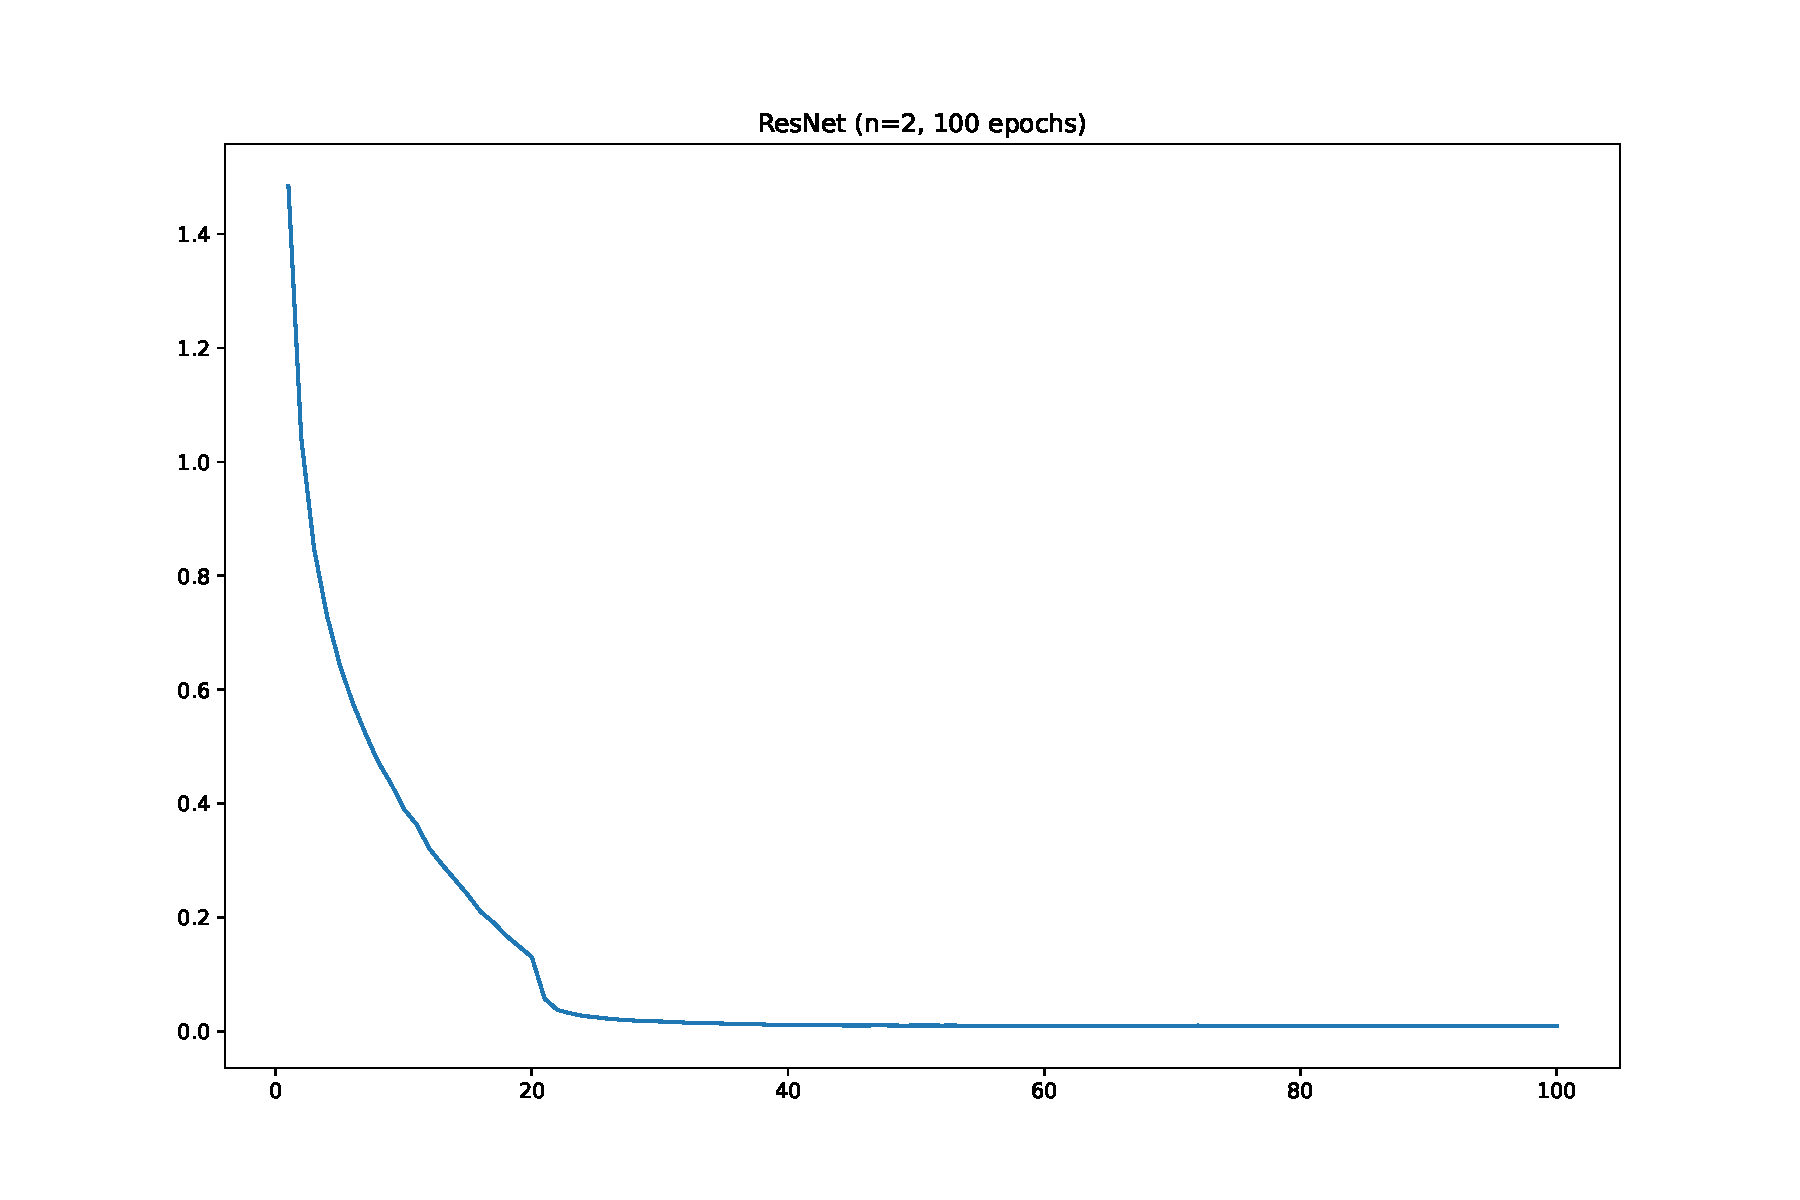
\includegraphics[width=0.7\textwidth]{../ResNet/q1_part2.pdf}
\end{figure}

\begin{figure}[!htbp]
    \centering
    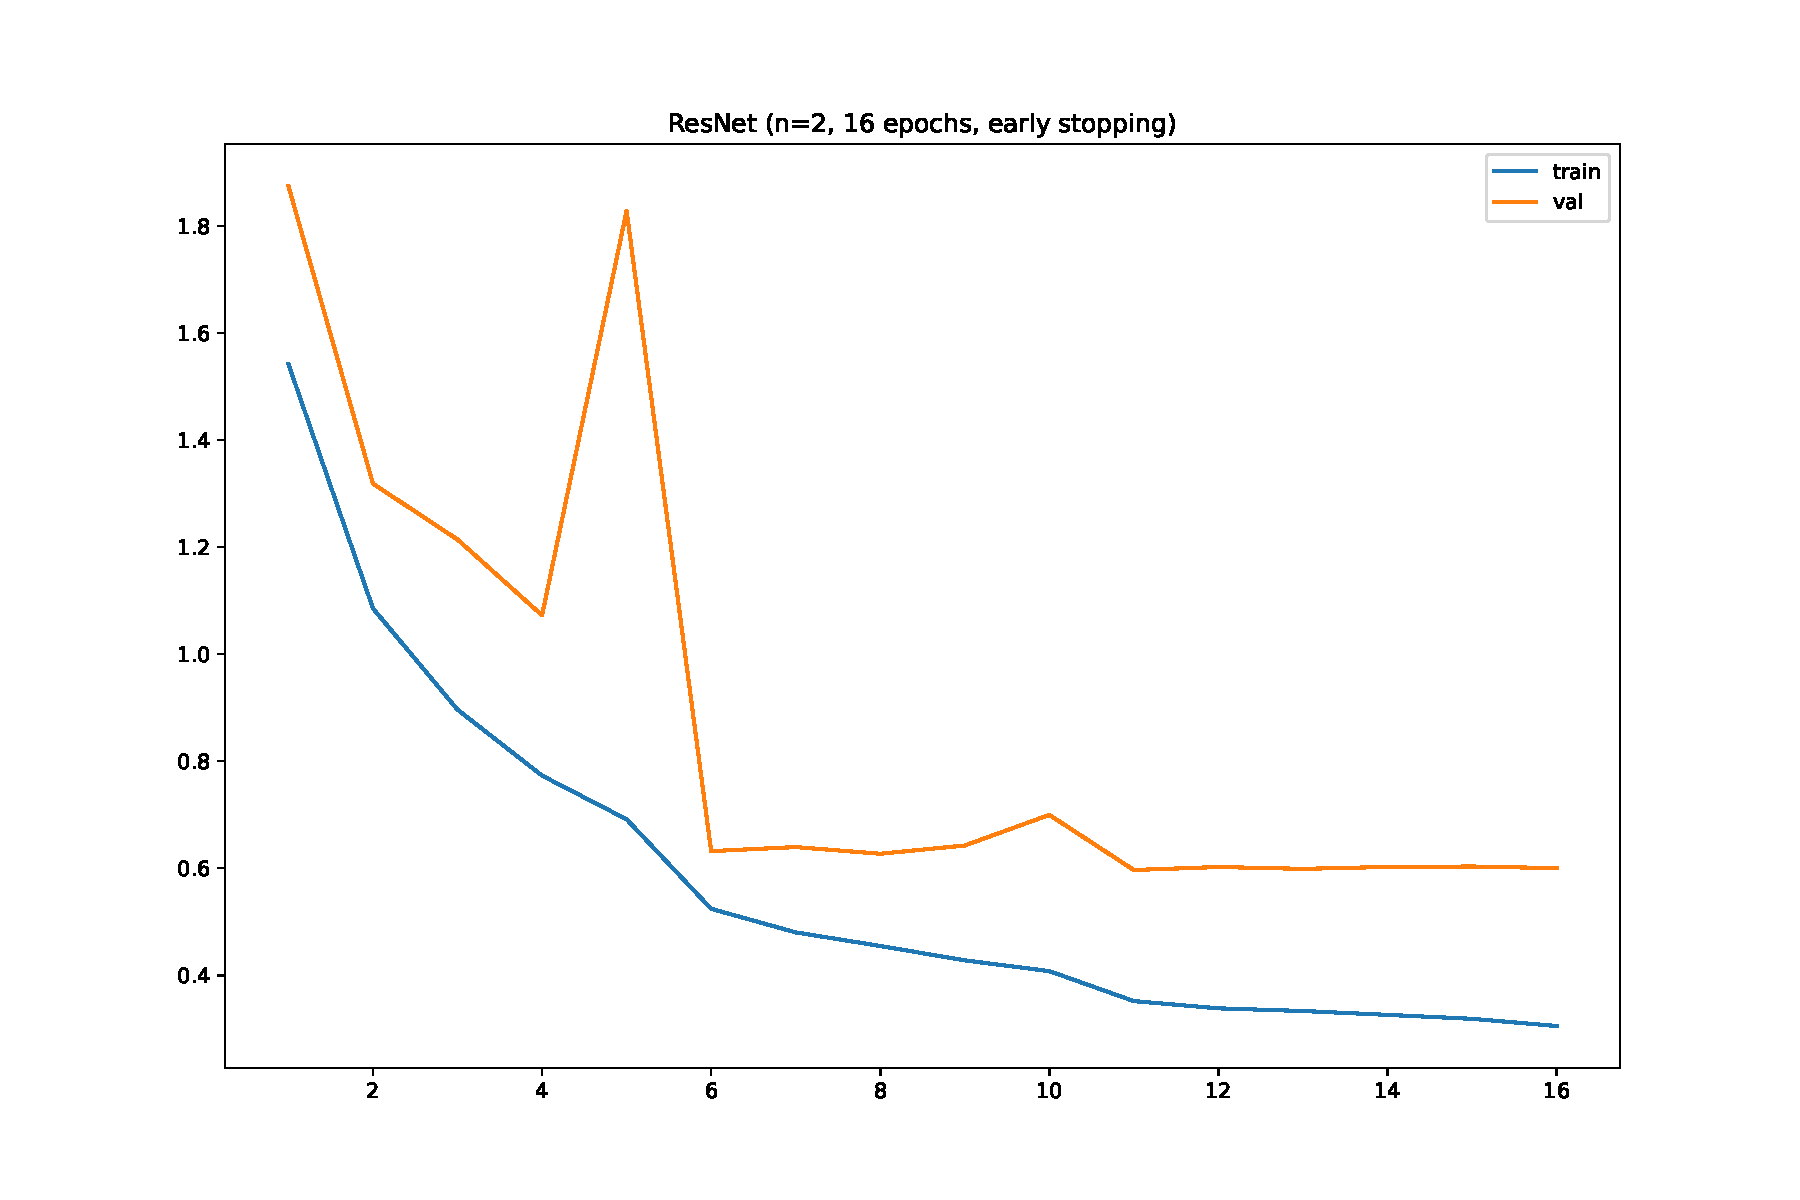
\includegraphics[width=0.7\textwidth]{../ResNet/q1_part3.pdf}
\end{figure}

\begin{center}
\begin{tabular}{|l|c|c|c|}
    \hline
    & Accuracy & F1 micro & F1 macro \\ 
    \hline
    train & 0.916 & 0.916 & 0.916 \\
    val & 0.797 & 0.797 & 0.796 \\
    test & 0.791 & 0.791 & 0.790 \\
    \hline
\end{tabular}
\end{center}

\subsection{Impact of Normalization}

\begin{center}
\begin{tabular}{|l|r|c|c|c|}
    \hline
    Norm & set & Accuracy & F1 micro & F1 macro \\
    \hline
    \multirow{3}{*}{bn (torch)}%
    & train & 0.913 & 0.913 & 0.913 \\
    & val & 0.791 & 0.791 & 0.790 \\
    & test & 0.783 & 0.783 & 0.783 \\
    \hline

    \hline
    \multirow{3}{*}{bn}%
    & train & 0.913 & 0.913 & 0.913 \\
    & val & 0.782 & 0.782 & 0.781 \\
    & test & 0.785 & 0.785 & 0.785 \\
    \hline

    \hline
    \multirow{3}{*}{in}%
    & train & 0.725 & 0.725 & 0.724 \\
    & val & 0.684 & 0.684 & 0.682 \\
    & test & 0.669 & 0.669 & 0.667 \\
    \hline

    \hline
    \multirow{3}{*}{bin}%
    & train & 0.933 & 0.933 & 0.932 \\
    & val & 0.788 & 0.788 & 0.787 \\
    & test & 0.780 & 0.780 & 0.780 \\
    \hline

    \hline
    \multirow{3}{*}{ln}%
    & train & 0.766 & 0.766 & 0.765 \\
    & val & 0.725 & 0.725 & 0.723 \\
    & test & 0.727 & 0.727 & 0.725 \\
    \hline

    \hline
    \multirow{3}{*}{gn}%
    & train & 0.757 & 0.757 & 0.756 \\
    & val & 0.706 & 0.706 & 0.705 \\
    & test & 0.699 & 0.699 & 0.697 \\
    \hline

    \hline
    \multirow{3}{*}{nn}%
    & train & 0.737 & 0.737 & 0.736 \\
    & val & 0.714 & 0.714 & 0.712 \\
    & test & 0.706 & 0.706 & 0.705 \\
    \hline
\end{tabular}

\end{center}

\begin{center}
    \begin{figure}[!htbp]
    \centering
    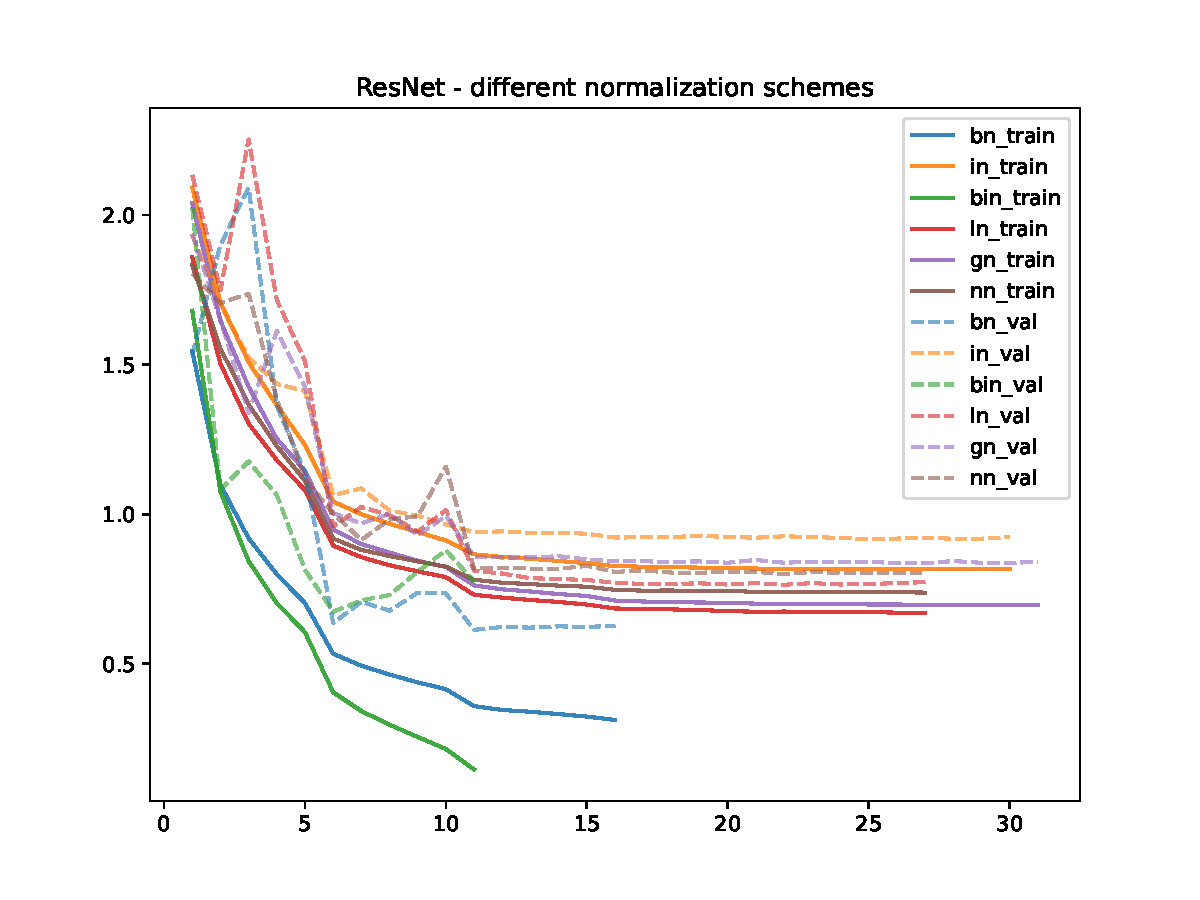
\includegraphics[width=0.7\textwidth]{../ResNet/q2_part3.pdf}
\end{figure}

\end{center}

\end{document}
